%%% generic article type (pdf)latex file
%%% use together with Makefile

\documentclass[letterpaper]{scrartcl}
\usepackage{graphicx}
\usepackage{amsmath,amsfonts,amsthm,amsbsy}
\usepackage{eufrak}
\usepackage{mathabx}
\usepackage{courier}
\usepackage{url}
\usepackage{color}
\usepackage[usenames,dvipsnames,svgnames,table]{xcolor}
\usepackage{hyperref}
\hypersetup{
     colorlinks   = true,
     urlcolor     = blue,
     linkcolor    = red,
     citecolor    = black
}


\usepackage{enumitem}
\usepackage{booktabs}
\usepackage{cprotect}
\usepackage{minted}

%\usepackage{wrapfig}
%\usepackage{subfig}
%\usepackage[format=plain,labelsep=period,font=small,labelfont=bf]{caption}

%------------------------------------------------------------
% makeup
%
\newcommand{\anumber}{11}
%
%------------------------------------------------------------
\newcommand{\anum}{\anumber}

% hyperref https://en.wikibooks.org/wiki/LaTeX/Hyperlinks#.5Chref
\urlstyle{same}


%% not working yet...
\newcounter{TotalPoints}
\newcounter{TotalBonus}

\newcommand{\BONUS}{\textsc{Bonus: }}
\newcommand{\bonus}[1]{\textbf{[bonus +#1*]}\stepcounter{TotalBonus}}
\newcommand{\points}[1]{\textbf{[#1 points]}\stepcounter{TotalPoints}}
\newenvironment{enuma}{\begin{enumerate}[label=(\alph*)]}{\end{enumerate}}
\newenvironment{enumi}{\begin{enumerate}[label=(\roman*)]}{\end{enumerate}}
\newenvironment{solution}{\par\noindent\P{} }{\ \qedsymbol}

\renewcommand{\vec}[1]{\ensuremath{\mathbf{#1}}}
\newcommand{\pd}[3][]{\left(\frac{\partial #2}{\partial #3}\right)_{#1}}




\begin{document}
%\maketitle

\setcounter{section}{\anumber}
\addtocounter{section}{-1}
\section{ --- PHY 494:  Assignment \anumber{} (20 points total)}

\noindent Due Wednesday, April 24, 2018, 11:59pm.

\noindent
\fbox{\parbox{\linewidth}{Submission is to your \textbf{private
      GitHub repository}.}}

Enter the repository and run the script
\texttt{scripts/update.sh} (replace \emph{YourGitHubUsername} with
your GitHub username):
\begin{minted}{bash}
cd assignments-2018-YourGitHubUsername
bash ./scripts/update.sh 
\end{minted} 
It should create three subdirectories\footnote{If the script fails,
  file an issue in the
  \href{https://github.com/ASU-CompMethodsPhysics-PHY494/PHY494-assignments-skeleton/issues}{Issue
    Tracker for PHY494-assignments-skeleton} and just create the
  directories manually.} \texttt{assignment\_\anum{}/Submission},
\texttt{assignment\_\anum{}/Grade}, and
\texttt{assignment\_\anum{}/Work} and also pull in the PDF of the
makeup and an additional file.

To submit your makeup assignment, commit and push Python code inside
the \texttt{assignment\_\anum{}/Submission} directory. \emph{Commit
  any other additional files exactly as required in the problems.}

Code will be tested against the unit tests in
\texttt{test\_capacitor.py}. The grade will be approximately
proportional to the number of tests that pass successfully so your
code \emph{must} be able run under the tests.



\subsection{Numerical solution of the plate capacitor potential (20 points)}
\label{sec:capacitor}

\begin{figure}[!h]
  \centering
  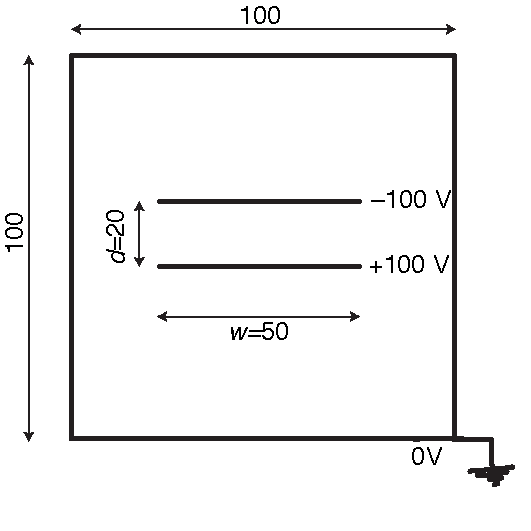
\includegraphics[width=0.5\linewidth]{CapacitorInBox.pdf}
  \caption{Schematic of the capacitor in the grounded box problem
    (2D). The capacitor is centered in the box. The capacitor plates
    are thin, conducting sheets of metal that are held at potential
    +100 V and -100 V, respectively.}
  \label{fig:capacitor}
\end{figure}

Compute the electrostatic potential of a plate capacitor in a grounded
box, shown in Fig.~\ref{fig:capacitor}. Solve the problem in 2D. The
square box has sides of length 100. Consider the capacitor plates to
be conducting, very thin sheets of metal. The plates are held at an
electric potential of +100~V and -100~V. The plates are $w=50$ units wide
and located at a distance $d=20$. The capacitor is centered inside the
box.

Submit your code as a python module \texttt{capacitor.py}. In
particular, you should have the following functions:\footnote{See also
  \href{https://asu-compmethodsphysics-phy494.github.io/ASU-PHY494//2019/04/11/16_PDEs/}{Lesson
    16} and in particular the notebook
  \href{https://nbviewer.jupyter.org/github/ASU-CompMethodsPhysics-PHY494/PHY494-resources/blob/master/16_PDEs/16_PDEs-2.ipynb}{16\_PDEs-2.ipynb}.}
\begin{description}
\item[\texttt{set\_boundaries(Phi)}] Given the potential on the
  lattice, enforce the boundary conditions by setting the appropriate
  lattice points to the prescribed values.
\item[\texttt{calculate\_phi\_capacitor(Max\_iter=10000, tol=1e-3)}] This
  function should calculate the potential $\Phi$ on the lattice. It
  needs to take at least the two keyword arguments \texttt{Max\_iter}
  to set the maximum number of iterations and \texttt{tol} to set the
  convergence criterion.

  You must implement a convergence check: consider the solution
  converged when the Frobenius norm
  \begin{gather}
    ||\Phi^{\text{new}} - \Phi^{\text{old}}|| :=
    \sqrt{\sum_{i=1}^{M}\sum_{j=1}^{N} \left|\Phi^{\text{new}}_{ij} -
        \Phi^{\text{old}}_{ij}\right|^{2}}
    \label{eq:Frobeniusnorm}    
  \end{gather}
  is less than the set tolerance \texttt{tol}. Report the
  number of iterations that were required. Also report if convergence
  was not achieved within \texttt{Max\_iter} iterations.

  The function \emph{must} return the potential $\Phi$ as a numpy
  array of dimensions $(100, 100)$.
\end{description}
It must be possible to run these functions as
\begin{minted}{python}
import capacitor
Phi = capacitor.calculate_phi_capacitor(Max_iter=2000, tol=1)
\end{minted}

Start from the skeleton code in \texttt{capacitor.py} to ensure that
your functions adhere to the prescribed interface.\footnote{The
  skeleton code contains a optimized function
  \texttt{Laplace\_Gauss\_Seidel\_odd\_even()} which replaces the
  Gauss-Seidel code from the lecture. It runs 50 times faster so you
  are advised to use it\dots but you may use the slower code, if you
  prefer. The original code (as developed in class) is in the function
  \texttt{Laplace\_Gauss\_Seidel()}.}

Specifically, you need to fullfil the following objectives:
\begin{enuma}
\item Your code must produce correct results, as tested with
  \texttt{test\_capacitor.py}. You can run these tests yourself with
\begin{minted}{bash}
pytest -v test_capacitor.py
\end{minted}
  (in the same directory as your \texttt{capacitor.py}). \points{15}
\item Converge your results to \texttt{tol = 1e-3}. 
  Include in your submission:
  \begin{enumerate}
  \item Report how many iterations you required for
    convergence. Simply write the number in a \emph{textfile}
    \texttt{iterations.txt} \points{3}
  \item Make a 3D plot of the potential (you can use
    \texttt{capacitor.plot\_phi(Phi)}) \points{1}
  \item Make a 2D plot of the initial potential (boundary conditions)
    and of the final converged solution (you can use
    \texttt{capacitor.plot\_panel(Phi)}) \points{1}
  \end{enumerate}
\end{enuma}

Note: You don't have to submit any notebooks or written
text. It will be sufficient to submit
\begin{itemize}
\item \texttt{capacitor.py}
\item \texttt{iterations.txt}
\item \texttt{capacitor\_potential\_2d.pdf} and
  \texttt{capacitor\_potential\_3d.pdf} (these are the default filenames
  when using the functions in \texttt{capacitor.py}).
\end{itemize}

\end{document}

%%% Local Variables: 
%%% mode: latex
%%% TeX-master: t
%%% End: 
